
\section{\blue{\sysplus：每个标记一条小通路}}
\label{sec:method}

\blue{\sysplus 是一个拥有三个标记与三条小通路的模型，每条通路预测第\ref{sec:motivations}节中窗口形式 $X\approx\ell\,\one^\top+a\,s^\top$ 的一部分（图\ref{fig:la_overview}）。\emph{相位通路}是一个基于相位的路由 Transformer，读取相位标记并预测每个相位，从而得到形状 $s$（第\ref{subsec:phase-network}节）。\emph{水平通路}读取水平标记，经由一个到固定偏移、倾斜与曲率轮廓的秩三映射预测水平项（第\ref{sec:ext_level}节）。\emph{振幅通路}以水平驱动的因子缩放相位预测的周期内部分（第\ref{sec:ext_modulation}节）。随后两个门控将已被振幅通路重缩放的相位预测与水平通路预测融合（第\ref{sec:ext_init}节）。因此一个水平标记同时驱动水平与振幅，三条通路产生一个预测。这些通路之所以小，是因为各自承载的内容是低维的：在最大的基准 Traffic 上，相位通路约需 1.2K 参数，水平与振幅通路至多再增加约 2.1K（第\ref{sec:complexity}节与第\ref{sec:exp_efficiency}节）。}

\blue{\fakeparagraph{问题设定}
\sysplus 是通道独立的}~\citep{nie2023patchtst, zeng2023dlinear}\blue{：一个共享模型分别预测每个传感器的序列，因此它在传感器网络上的代价等于单传感器代价乘以传感器数量。以下我们省略通道维；数据集的 $C$ 个通道共享一个模型。}预测的目标是从输入序列 $\mathbf{X}\in\mathbb{R}^{L_{\text{in}}}$ 预测未来轨迹 $\mathbf{Y}\in\mathbb{R}^{L_{\text{out}}}$，其中 $L_{\text{in}}$ 与 $L_{\text{out}}$ 分别表示输入长度与输出长度。

\begin{figure*}[t]
\centering
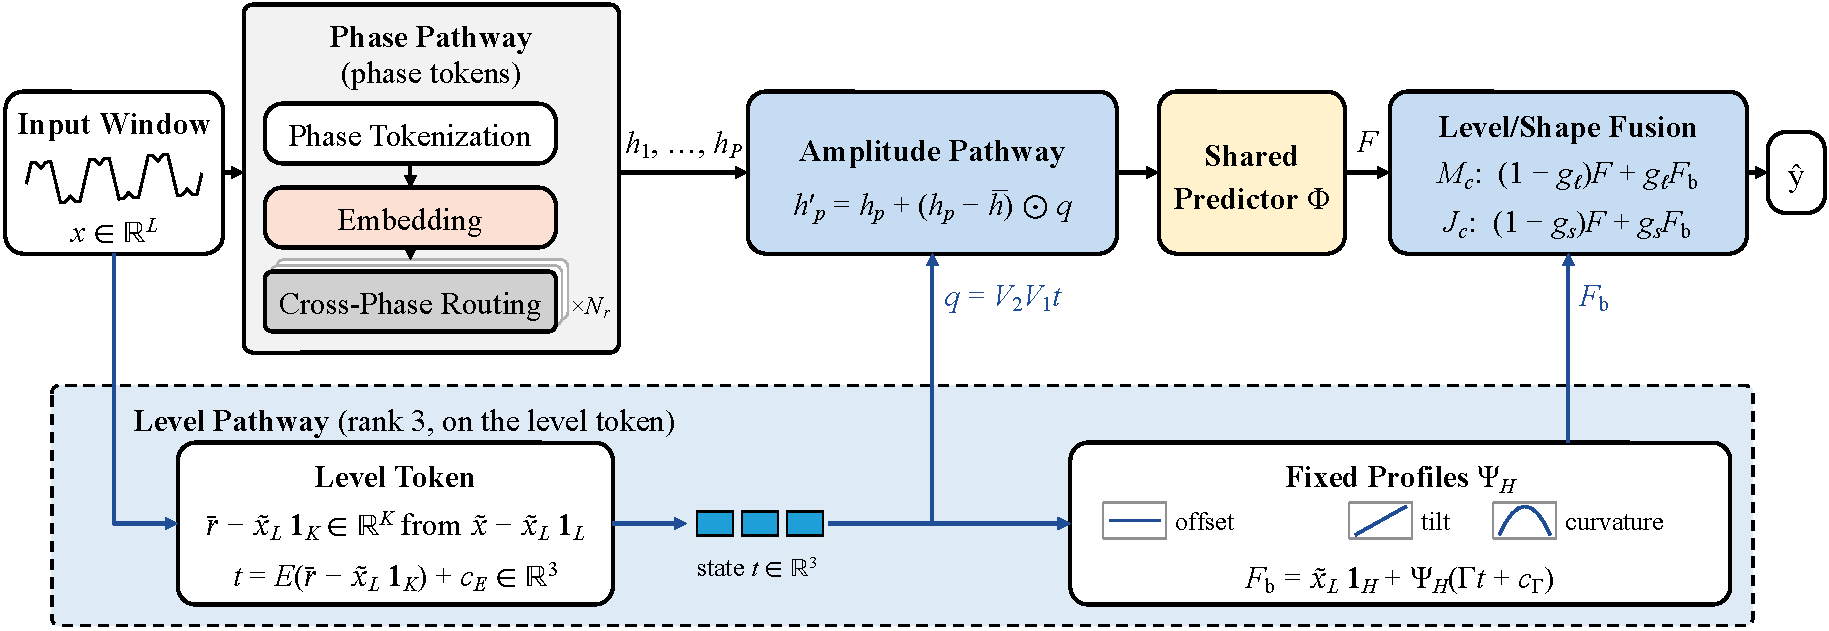
\includegraphics[width=\textwidth]{figures/la_overview.pdf}
\caption{\blue{\sysplus：三个标记、三条小通路、一个预测。相位通路嵌入相位标记，并通过 $N_r$ 层跨相位路由层将其精炼为最终相位隐变量 $h_1,\dots,h_P$；在振幅通路对其重缩放之后，共享预测器 $\Phi$ 将其解码为相位预测 $F$。水平通路（下方）将水平标记（即锚定的周期均值）映射为三维状态 $t$，并将其映射到偏移、倾斜与曲率轮廓 $\Psi_H$ 上，得到水平通路预测 $F_{\mathrm b}$。振幅通路由同一状态 $t$ 计算振幅标记 $q$，并以 $\one+q$（在相位上中心化）缩放相位隐变量的周期内部分。两个门控融合 $F$ 与 $F_{\mathrm b}$ 的周期水平与周期内形状。图\ref{fig:overview}给出相位通路的细节。}}
\label{fig:la_overview}
\end{figure*}

\begin{figure*}[t]
    \centering
    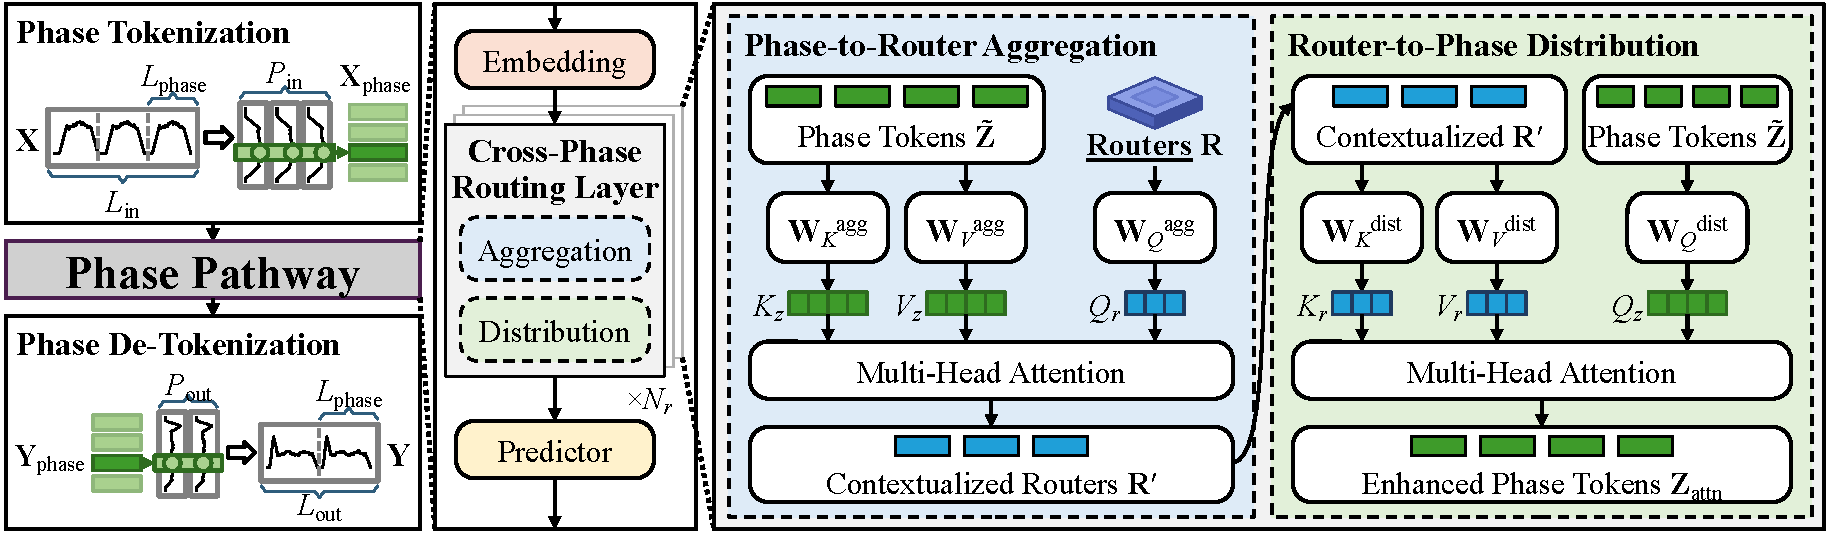
\includegraphics[width=\textwidth]{figures/phaseformer_overview.pdf}
    \caption{\blue{\sysplus 的相位通路：相位标记化与去标记化（左）；嵌入层、$N_r$ 层跨相位路由层与共享预测器（中）；以及路由层内部，若干路由器从所有相位收集消息再分发回去（右）。}}
    \label{fig:overview}
\end{figure*}

\subsection{\blue{从窗口到三个标记}}
\label{subsec:preprocessing}
\fakeparagraph{归一化与去归一化}
遵循 \cite{kim2021reversible}，我们用输入的估计均值与标准差对其进行归一化，并将预测去归一化到原始尺度。\blue{该归一化（RevIN）将均值为 $\mu$、标准差为 $\sigma$ 的输入窗口 $x$ 映射为 $\tilde x=(x-\mu\one)/\sigma$，使 $\one^\top\tilde x=0$；该坐标系下的预测 $\hat{\tilde y}$ 去归一化为 $\hat y=\mu\one+\sigma\hat{\tilde y}$。}

\fakeparagraph{相位标记化与去标记化}
相位标记化将一维输入序列变换为二维的相位–周期矩阵，以供\blue{后续}处理。
反之，相位去标记化将预测的相位–周期矩阵重构回一维输出序列。
\revised{\blue{记 $L_{\text{phase}}$ 为周期长度，即一个周期所含的步数，我们也称其为相位长度；它由频域分析估计（\secref{sec:phase_length}）并保持固定。}}

为确保输入序列长度是 $L_{\text{phase}}$ 的整数倍，我们循环填充序列至长度 \blue{$P_{\text{in}}L_{\text{phase}}$}，其中 $P_{\text{in}} = \left\lceil \frac{L_{\text{in}}}{L_{\text{phase}}} \right\rceil.$ \blue{是 $L_{\text{phase}}$ 整数倍的输入长度无需填充，建议尽可能采用。}
如\figref{fig:overview}所示，填充后的序列 $\mathbf{X}$ 随后被重塑为相位–周期矩阵 $\mathbf{X}_{\text{phase}} \in \mathbb{R}^{L_{\text{phase}} \times P_{\text{in}}}$，其中每个元素 \blue{$\mathbf{X}_{\text{phase}}[p, k]$ 对应第 $k$ 个周期中第 $p$ 个相位处的观测}。
\blue{去标记化将这一重塑逆转。}

\blue{
\fakeparagraph{记号}
我们简记 $P=\Lp$ 为周期，$K=\Pin$ 与 $K'=\Pout$ 为输入与输出周期数，$L=L_{\text{in}}=KP$ 与 $H=L_{\text{out}}=K'P$ 为输入长度与预测时域。对频域分析找到的周期，实验的输入长度与每个预测时域都是整数个周期，因此不会发生填充。折叠后的归一化窗口 $\tilde X\in\mathbb R^{K\times P}$（即 $\tilde x$ 的相位–周期矩阵的转置）每周期一行；它就是第\ref{sec:motivations}节中 $D=K$ 个周期、$H=P$ 个相位的矩阵 $X$，此后 $H$ 表示预测时域。第\ref{subsec:phase-network}节与第\ref{sec:complexity}节使用符号 $\Lp$、$\Pin$ 与 $\Pout$，它们同样适用于填充后的输入。

\fakeparagraph{三个标记}
三个标记对应\equref{eq:three_parts}的三个部分。
\begin{itemize}[leftmargin=1.2em,itemsep=0.1em,topsep=0.2em]
\item \emph{相位标记}是 $\tilde X$ 的列 $\tilde x_p\in\mathbb R^K$，每个相位一个。除去噪声，每个列都等于 $\ell+s_p\,a$，因此它们共同以稳定子空间中坐标的形式携带形状 $s$（第\ref{sec:mot_stability}节）。
\item \emph{水平标记}是窗口的周期水平向量 $\ell$，以窗口的最后一个值 $\tilde x_L$ 为基准度量，
\begin{equation}
\bar r-\tilde x_L\one_K,\qquad \bar r=\tfrac1P\tilde X\one_P\in\mathbb R^K ,
\label{eq:level_token}
\end{equation}
每周期一个数。锚点使其在归一化坐标下具有平移不变性：向 $\tilde x$ 加 $c\one_L$ 不改变水平标记。
\item \emph{振幅标记}是由水平通路的状态计算得到的尺度 $q\in\mathbb R^d$（\equref{eq:la_modulation}）。它是振幅因子 $a$ 的隐变量形式：振幅通路以 $\one+q$ 缩放相位隐变量的周期内部分，因此均匀的 $q=q_1\one_d$ 以单一因子 $1+q_1$ 缩放相位预测的周期内部分。它无需自己的输入，因为振幅跟随水平（第\ref{sec:mot_changes}节）。
\end{itemize}
}

% --------------------------------------------------------------------
\subsection{\blue{相位通路：基于相位的路由 Transformer}}
\label{subsec:phase-network}

\blue{相位通路预测形状。它是一个基于相位的路由 Transformer，是 \sysplus 中唯一使用注意力的部分，由相位标记预测每个相位。}
如\figref{fig:overview}所示，\blue{相位通路}首先对相位标记施加嵌入层，然后通过 \blue{$N_r$ 层}跨相位路由层对其进行精炼，最后经共享预测器将其映射到目标。

% ---------------- embedding ----------------
\subsubsection{嵌入层}
嵌入层将相位标记 $\mathbf{X}_{\text{phase}}$ 投影到低维表示空间，从而能够从常受扰动污染的原始观测中提取信息成分。
形式上，对每个相位索引 \blue{$p \in \{1,\dots,L_{\text{phase}}\}$，其对应的相位标记 $\mathbf{X}_{\text{phase}}[p, :]$}通过\blue{一个仿射映射 $f_{\theta}$，$\theta=(W_e,b_e)$，其权重为 $W_e\in\mathbb R^{d\times\Pin}$、偏置为 $b_e\in\mathbb R^d$，并后接一个 LayerNorm $\LN_e$~\citep{ba2016layernorm}}，被映射为 $d$ 维表示：
\begin{equation}
\mathbf{Z}
= \blue{\LN_e\big(}f_{\theta}\!\left(\mathbf{X}_{\text{phase}}\right)\blue{\big)}\in \mathbb{R}^{L_{\text{phase}}\times d}\blue{.}
\end{equation}

为更好地刻画相位之间的时间顺序，遵循 \cite{liu2023spatio}，我们引入一组可学习的位置嵌入 $\mathbf{E}_{\text{pos}}\in\mathbb{R}^{L_{\text{phase}}\times d}$\blue{，以编码每个相位在周期内的位置}。
这些嵌入逐相位地加到 $\mathbf{Z}$ 上，使每个相位表示都融入其位置信息：
\begin{equation}
\tilde{\mathbf{Z}}=\mathbf{Z}+\mathbf{E}_{\text{pos}}.
\end{equation}
所得的 $\tilde{\mathbf{Z}}$ 随后被送入跨相位路由层，以进行更高层次的特征交互与预测\blue{；在层堆叠中，每一层都以这种方式将自身的位置嵌入加到其输入上}。

% ---------------- Attention ----------------
\subsubsection{跨相位路由层}

\blue{相位标记之间需要交换信息，因为没有任何单个相位标记持有周期形状，而它们张成低维子空间（洞察~2，第\ref{sec:mot_stability}节），因此少量中介即可完成交换。}我们引入一组可学习的路由器 $\mathbf{R}\in\mathbb{R}^{M\times d}$，充任跨相位信息交换的中介。
\revised{
\blue{该设计沿袭已有的路由式架构~\citep{jaegle2021perceiver, zhang2023crossformer}，且路由器利用了}\emph{相位对齐标记固有的低秩结构}。
\blue{跨相位路由将自注意力的二次代价降为关于相位个数的线性代价，同时每个相位仍能与所有其他相位交换信息。}
}

跨相位路由包含两步：
(i) \emph{相位到路由器聚合}，将相位表示中的信息选择性地压缩进紧凑的路由器集合；(ii) \emph{路由器到相位分发}，将聚合的跨相位信息从路由器选择性地传播回相位表示。两步均由交叉注意力实现。

\fakeparagraph{相位到路由器聚合}
路由器关注相位表示以提取上下文信息，得到上下文化路由器嵌入
\blue{$\mathbf{R}'\in\mathbb{R}^{M\times d}$}。
具体而言，路由器充当查询，相位提供键与值。投影矩阵
$\mathbf{W}_Q^{\text{agg}},\mathbf{W}_K^{\text{agg}},\mathbf{W}_V^{\text{agg}}\in\mathbb{R}^{d\times d}$
分别将表示映射到查询、键与值空间：
\begin{equation}
\mathbf{Q}_r=\mathbf{R}\mathbf{W}_Q^{\text{agg}},\quad
\mathbf{K}_z=\tilde{\mathbf{Z}}\mathbf{W}_K^{\text{agg}},\quad
\mathbf{V}_z=\tilde{\mathbf{Z}}\mathbf{W}_V^{\text{agg}}.
\end{equation}
随后通过 \blue{$n_h$} 个头的多头注意力（MHA）得到聚合的路由器嵌入：
\begin{equation}
\blue{\mathbf{R}'}=\mathrm{MHA}\!\left(\mathbf{Q}_r,\mathbf{K}_z,\mathbf{V}_z\right).
\end{equation}

\fakeparagraph{路由器到相位分发}
路由器中聚合的信息随后被重新分发到相位表示，从而实现跨相位信息流动。此步中，相位表示充当查询，路由器提供键与值，得到精炼的相位表示 $\mathbf{Z}_{\text{attn}}$。分发使用投影矩阵 $\mathbf{W}_Q^{\text{dist}}, \mathbf{W}_K^{\text{dist}}, \mathbf{W}_V^{\text{dist}}\in\mathbb{R}^{d\times d}$：
\begin{equation}
\begin{gathered}
\mathbf{Q}_z=\tilde{\mathbf{Z}}\mathbf{W}_Q^{\text{dist}},\quad
\mathbf{K}_r=\blue{\mathbf{R}'}\mathbf{W}_K^{\text{dist}},\quad
\mathbf{V}_r=\blue{\mathbf{R}'}\mathbf{W}_V^{\text{dist}},\\
\mathbf{Z}_{\text{attn}}=\mathrm{MHA}\!\left(\mathbf{Q}_z,\mathbf{K}_r,\mathbf{V}_r\right).
\end{gathered}
\end{equation}
该机制在恢复相位级分辨率的同时，通过上下文化路由器在相位之间施加一致性。
最终，每个相位表示\blue{都经由路由器、分两步}关注所有其他相位。
\blue{路由层将这两步与残差连接、两个 LayerNorm 和一个 MLP 组合起来：记 $z_p$ 与 $m_p$ 为层输入（首层为 $\tilde{\mathbf Z}$）与 $\mathbf Z_{\text{attn}}$ 的第 $p$ 行，它计算 $o_p=\LN_1(z_p+m_p)$ 并输出 $h_p=\LN_2\big(o_p+\mathrm{MLP}(o_p)\big)$。每个 LayerNorm 在 $d$ 个特征上对其输入做中心化，将其重缩放到单位均方根，并施加可学习的增益 $\gamma_i$ 与偏置 $\beta_i$：$\LN_i(u)=\gamma_i\odot\varsigma+\beta_i$，其中 $\varsigma=J_du/(\|J_du\|^2/d+\epsilon)^{1/2}$、$J_d=I_d-\tfrac1d\one\one^\top$。因此对任意输入有 $\|\varsigma\|<\sqrt d$；又因为 $\LN_2$ 是每个路由层的最后一个操作，每个最终相位隐变量都是有界的。该界把每个相位预测的水平与周期内振幅限制在第\ref{sec:theory}节的两个包络之内，这正是水平标记与振幅标记各自拥有通路的原因：水平通路绕过 $\LN_2$，振幅通路对其输出进行重缩放。附录\ref{app:proofs}给出完整的层与层堆叠。}


% ---------------- predictor ----------------
\subsubsection{预测器}

预测器基于精炼后的表示，同时为所有相位生成长度为 $P_{\text{out}}$ 的多步预测。预测器以最后一个跨相位路由层输出的\blue{相位表示 $\mathbf Z_{\text{out}}=[h_1;\dots;h_{L_{\text{phase}}}]\in\mathbb{R}^{L_{\text{phase}}\times d}$}\blue{，即\emph{最终相位隐变量}}为输入，实现为\blue{一个仿射}映射\blue{$g_{\Phi}$}，由\blue{权重 $\Phi\in\mathbb{R}^{P_{\text{out}}\times d}$ 与偏置 $c_\Phi\in\mathbb{R}^{P_{\text{out}}}$ 参数化，并施加于每个相位}：
\begin{equation}
\begin{gathered}
\mathbf{Y}_{\text{phase}} = \blue{g_{\Phi}(\mathbf Z_{\text{out}})}
\in \mathbb{R}^{L_{\text{phase}}\times P_{\text{out}}}\blue{,}\\
\blue{F_p=\Phi h_p+c_\Phi\in\mathbb R^{P_{\text{out}}}.}
\end{gathered}
\label{eq:predictor}
\end{equation}
所有相位共享同一组预测器参数，这保证了跨相位的一致性并减少了可训练参数量\blue{：每个相位都由同一映射解码，因此各相位预测的差异仅来自其隐变量}。
\blue{在第\ref{subsec:preprocessing}节的记号下，$\mathbf Y_{\text{phase}}$ 的第 $p$ 行保存相位 $p$ 的 $K'$ 个未来值 $F_p$（归一化单位），对 $\mathbf Y_{\text{phase}}$ 去标记化即得\emph{相位预测} $F\in\mathbb R^H$；从相位标记到 $F$ 的计算就是相位通路。仅含相位通路的模型，即 \sysplus 的\emph{仅相位变体}，预测 $\hat{\tilde y}=F$ 并对其去归一化。在 \sysplus 中，预测器在振幅通路之后读取最终相位隐变量（第\ref{sec:ext_modulation}节），$F$ 与水平预测融合（第\ref{sec:ext_init}节）。}


\blue{
\subsection{水平通路}
\label{sec:ext_level}

水平通路预测水平项。窗口的水平由其周期均值承载，且水平的预测在整个预测时域上是平滑的（在季节随机游走下为常数，引理\ref{lem:bayes}）。因此水平通路只读取水平标记（\equref{eq:level_token}）并写到少数几条平滑轮廓上（图\ref{fig:la_overview}下方）。它将水平标记映射为三维状态，
\begin{equation}
\begin{gathered}
t=E(\bar r-\tilde x_L\one_K)+c_E\in\mathbb R^3,\\
F_{\mathrm b}=\tilde x_L\one_H+\Psi_H\,(\Gamma t+c_\Gamma),
\end{gathered}
\label{eq:branch}
\end{equation}
其中 $\Psi_H=[\one_H,\psi_2,\psi_3]\in\mathbb R^{H\times3}$ 保存偏移、倾斜与曲率轮廓，即预测网格上 $0,1,2$ 次的离散正交多项式，并归一化到单位均方根，故其第一列为 $\one_H$，其余两列在预测时域上均值为零。$\Psi_H$ 是固定的；只有 $E\in\mathbb R^{3\times K}$、$c_E\in\mathbb R^3$、$\Gamma\in\mathbb R^{3\times3}$ 与 $c_\Gamma\in\mathbb R^3$ 是可学习的，共 $3K+15$ 个参数。借助锚点，水平通路是平移等变的：向 $\tilde x$ 加 $c\one_L$ 不改变 $t$，并给 $F_{\mathrm b}$ 加上 $c\one_H$。在标准季节模型下，相位通路无法企及的水平经由一个到少数固定预测时域轮廓的低秩映射进入（定理\ref{thm:complement}），第\ref{sec:exp_capacity}节证实这三条轮廓已经足够。水平通路直接读取窗口并在共享预测器之后融合，因此与相位预测不同，它绕过了相位通路的所有 LayerNorm，其水平不受定理\ref{thm:level_envelope}的水平包络约束。包络定理界定的是 $q=0$ 时的相位预测；振幅通路保持其水平界并重缩放其振幅界（命题\ref{prop:modulation}）。

\subsection{振幅通路}
\label{sec:ext_modulation}

振幅通路预测振幅因子。仅相位通路会将其预测的周期内振幅保持在一个固定界（即振幅包络）之下（定理\ref{thm:amplitude}(a)），而跟随水平的振幅会以水平缩放周期形状（\equref{eq:cycle_axis_changes}，图\ref{fig:coupling}）。因此振幅通路利用另外两条通路所提供的信息——形状与水平状态——并增加一个尺度。在共享预测器之前，振幅通路为每个最终相位隐变量 $h_p$ 加上其相对相位均值 $\bar h$ 的偏离，并按振幅标记 $q$ 逐元素缩放；$q$ 由水平通路的状态 $t$ 计算，该状态承载预测水平 $\hat\Lambda$（图\ref{fig:la_overview}上方中央）：
\begin{equation}
h'_p=h_p+(h_p-\bar h)\odot q,\qquad \bar h=\tfrac1P\textstyle\sum_ph_p,\qquad q=V_2V_1\,t,
\label{eq:la_modulation}
\end{equation}
其中 $V_1\in\mathbb R^{k_q\times3}$、$V_2\in\mathbb R^{d\times k_q}$、$k_q=\min(w,3,d)$，无偏置，共 $k_q(3+d)$ 个参数；宽度 $w$ 默认为 $2$。预测器随后以 $h'_p$ 代替 $h_p$，因此相位预测 $F$ 由调制后的隐变量计算得到。

\fakeparagraph{调制为何是中心化的}
由于\equref{eq:predictor}的预测器是共享且仿射的，$\Phi\bar h+c_\Phi$ 即相位预测的未来周期均值向量：$\bar h$ 是周期水平的隐变量对应物，$h_p-\bar h$ 则是周期内形状的隐变量对应物。偏离在相位上求和为零（中心化是在相位上进行的，而非像 LayerNorm 那样在 $d$ 个特征上），因此振幅通路只改变相位预测的周期内部分而不改变其周期均值（命题\ref{prop:modulation}(a)）；它从不移动水平通路设定的水平。均匀的 $q=q_1\one_d$ 以 $1+q_1$ 缩放该部分，而由预测水平 $\hat\Lambda$ 驱动的 $q$ 则提供乘性模型所需的水平驱动因子 $1+\alpha_w\hat\Lambda$（定理\ref{thm:amplitude}(b)，命题\ref{prop:modulation}(b)）。

\subsection{三条通路合为一个预测}
\label{sec:ext_init}

\fakeparagraph{门控融合}
设 $M_c$ 为 $\mathbb R^H$ 到在每个未来周期内取常值的向量子空间的正交投影，$J_c=I-M_c$：$M_c$ 把每个未来周期替换为其均值（周期水平），$J_c$ 保留周期内偏离（周期形状）；$\lev(v)=\tfrac1H\one^\top v$ 是预测 $v\in\mathbb R^H$ 的整体水平。对每个未来周期，融合预测通过两个独立的门控，分别从相位预测 $F$ 与水平通路预测 $F_{\mathrm b}$ 中取其水平与周期内形状，
\begin{equation}
\begin{gathered}
M_c\hat{\tilde y}=(1-g_\ell)M_cF+g_\ell M_cF_{\mathrm b},\\
J_c\hat{\tilde y}=(1-g_s)J_cF+g_sJ_cF_{\mathrm b},
\end{gathered}
\label{eq:fusion}
\end{equation}
其中 $g_\ell=\operatorname{sigmoid}(\omega)$、$g_s=\operatorname{sigmoid}(\omega+\delta)$，融合预测随后被去归一化。由于 $J_c\one_H=0$，水平通路只能通过其倾斜与曲率轮廓的周期内部分 $J_c\psi_2$ 与 $J_c\psi_3$ 进入周期内形状。门控是静态的：既不依赖输入也不依赖时间步。它们或逐通道学习，或在 $C$ 个通道间共享。

\fakeparagraph{整体模型}
综合\equref{eq:level_token}至\equref{eq:fusion}，\sysplus 对每个传感器计算
\begin{equation}
\begin{gathered}
t=E(\bar r-\tilde x_L\one_K)+c_E,\qquad q=V_2V_1t,\\
F_{\mathrm b}=\tilde x_L\one_H+\Psi_H(\Gamma t+c_\Gamma),\\
F_p=\Phi\big(h_p+(h_p-\bar h)\odot q\big)+c_\Phi,\\
\hat{\tilde y}=M_c\big[(1-g_\ell)F+g_\ell F_{\mathrm b}\big]\\
\qquad+J_c\big[(1-g_s)F+g_sF_{\mathrm b}\big],
\end{gathered}
\label{eq:forward}
\end{equation}
其中 $h_1,\dots,h_P$ 是相位通路的最终相位隐变量，$F$ 是 $F_1,\dots,F_P$ 的去标记化结果，且 $\hat y=\mu\one+\sigma\hat{\tilde y}$。相位标记决定隐变量，水平标记决定状态 $t$，而 $t$ 同时决定水平通路预测与振幅标记。

\fakeparagraph{简单的起始预测与嵌套变体}
水平与振幅通路从简单的预测起步：$\Gamma$ 与 $c_\Gamma$ 为零，因此水平通路初始预测最后一个值；$V_2$ 为零，因此振幅通路初始为恒等；两个门控从共同值 $g_0$ 出发，默认为 $0.2$（$\delta=0$）。标记消融的各变体是同一个模型的子模型：当 $V_2=0$ 时，\sysplus 恰好退化为\emph{相位–水平变体}，即仅含相位通路与水平通路，该变体在 $g_\ell,g_s\to0$ 时趋于仅相位变体。特别地，从同一随机状态、以相同的门控初始化构建的 \sysplus 及其相位–水平变体在初始化时预测完全相同，因此标记消融是在同一起始预测的基础上逐个添加标记。我们将以 $V_2=0$ 评估训练完成的 \sysplus 记作 \sysplus（振幅关闭）。
}

\subsection{\blue{效率：小通路，每传感器线性代价}}
\label{sec:complexity}

\blue{每条通路都很小，因为它承载的内容是低维的；而 \sysplus 没有跨传感器的操作，因此其单传感器代价决定了它在整个网络上的代价。对每个通道，相位通路的代价如下：}
相位嵌入层需要 $O(L_{\text{phase}} P_{\text{in}} d)$ 时间与 $O(L_{\text{phase}} d)$ 内存。
计算量占主导的跨相位路由层花费 $O((L_{\text{phase}}+M)d^2 + M L_{\text{phase}} d)$ 时间与 $O(\blue{n_h} M L_{\text{phase}} + (L_{\text{phase}}+M)d)$ 内存。
最后，预测器花费 $O(L_{\text{phase}} d P_{\text{out}})$ 时间与 $O(L_{\text{phase}} P_{\text{out}})$ 内存。
在 $\blue{N_r}$ \blue{个路由层上求和并代入} $P_{\text{in}}=\lceil L_{\text{in}}/L_{\text{phase}}\rceil$ 与
$P_{\text{out}}=\lceil L_{\text{out}}/L_{\text{phase}}\rceil$\blue{，端到端时间复杂度为}
\[
O\Big(\blue{N_r}\big((L_{\text{phase}}+M)d^2 + M L_{\text{phase}} d\big)
+ d(L_{\text{in}}+L_{\text{out}})\Big)\blue{.}
\]
如\blue{\secref{sec:mot_stability}}所考察，相位标记空间呈现\blue{固有的}低维结构，因此 $M$ 与 $d$ 可以取为固定的小数值。
这样，\blue{在层数固定时，}计算代价随输入长度 $L_{\text{in}}$ 与预测时域 $L_{\text{out}}$ \blue{线性}增长。

\blue{
\fakeparagraph{水平与振幅通路的代价}
采用\equref{eq:branch}的固定轮廓，水平通路在 $K=30$ 时有 $3K$（$E$）$+\,3$（$c_E$）$+\,9$（$\Gamma$）$+\,3$（$c_\Gamma$）$=105$ 个参数，振幅通路有 $k_q(3+d)$ 个，门控在 $C$ 个通道时为 $2C$ 个，共享时总共两个。在第\ref{subsec:preprocessing}节的记号下，水平通路每通道构造水平标记花费 $O(L)$、读出花费 $O(K+H)$，振幅通路花费 $O(Pd)$，二者相对相位通路都很小。在最大的基准 Traffic 上，相位通路约有 1.2K 参数，水平与振幅通路至多再增加约 2.1K，其中大部分为逐通道门控，且在 Traffic 与 Electricity 上其 FLOPs 不足相位通路的 0.25\%（第\ref{sec:exp_efficiency}节）。因此 \sysplus 的代价关于输入长度、预测时域与传感器数量均为线性，而且由于一个共享模型服务每个传感器，每次更新时每项节省都会在每个传感器上重复发生。
}
